\documentclass{article}

\usepackage[utf8]{inputenc}
\usepackage[danish]{babel}
\usepackage{float}
\usepackage{fancyhdr}
\usepackage{amsmath}
\usepackage{color}
\usepackage{listings}
\usepackage{graphicx}
\usepackage{pdfpages}
\usepackage{booktabs}
%\usepackage{enumitem}
\usepackage[a4paper, top = 1in, bottom = 1in, left=1in,right=1in]{geometry}

\title{Exercise 5}
\author{Peter Heilbo Ratgen}
\date{\today}

\begin{document}
\maketitle
\section{Data}
Vi laver en summering af variablen \texttt{ames\$Gr.Liv.Area}. 
\begin{lstlisting}
Min. 1st Qu.  Median    Mean 3rd Qu.    Max.
334    1126    1442    1500    1743    5642
\end{lstlisting}
Vi laver også et histogram over denne data.
\begin{figure}[H]
  \centering
  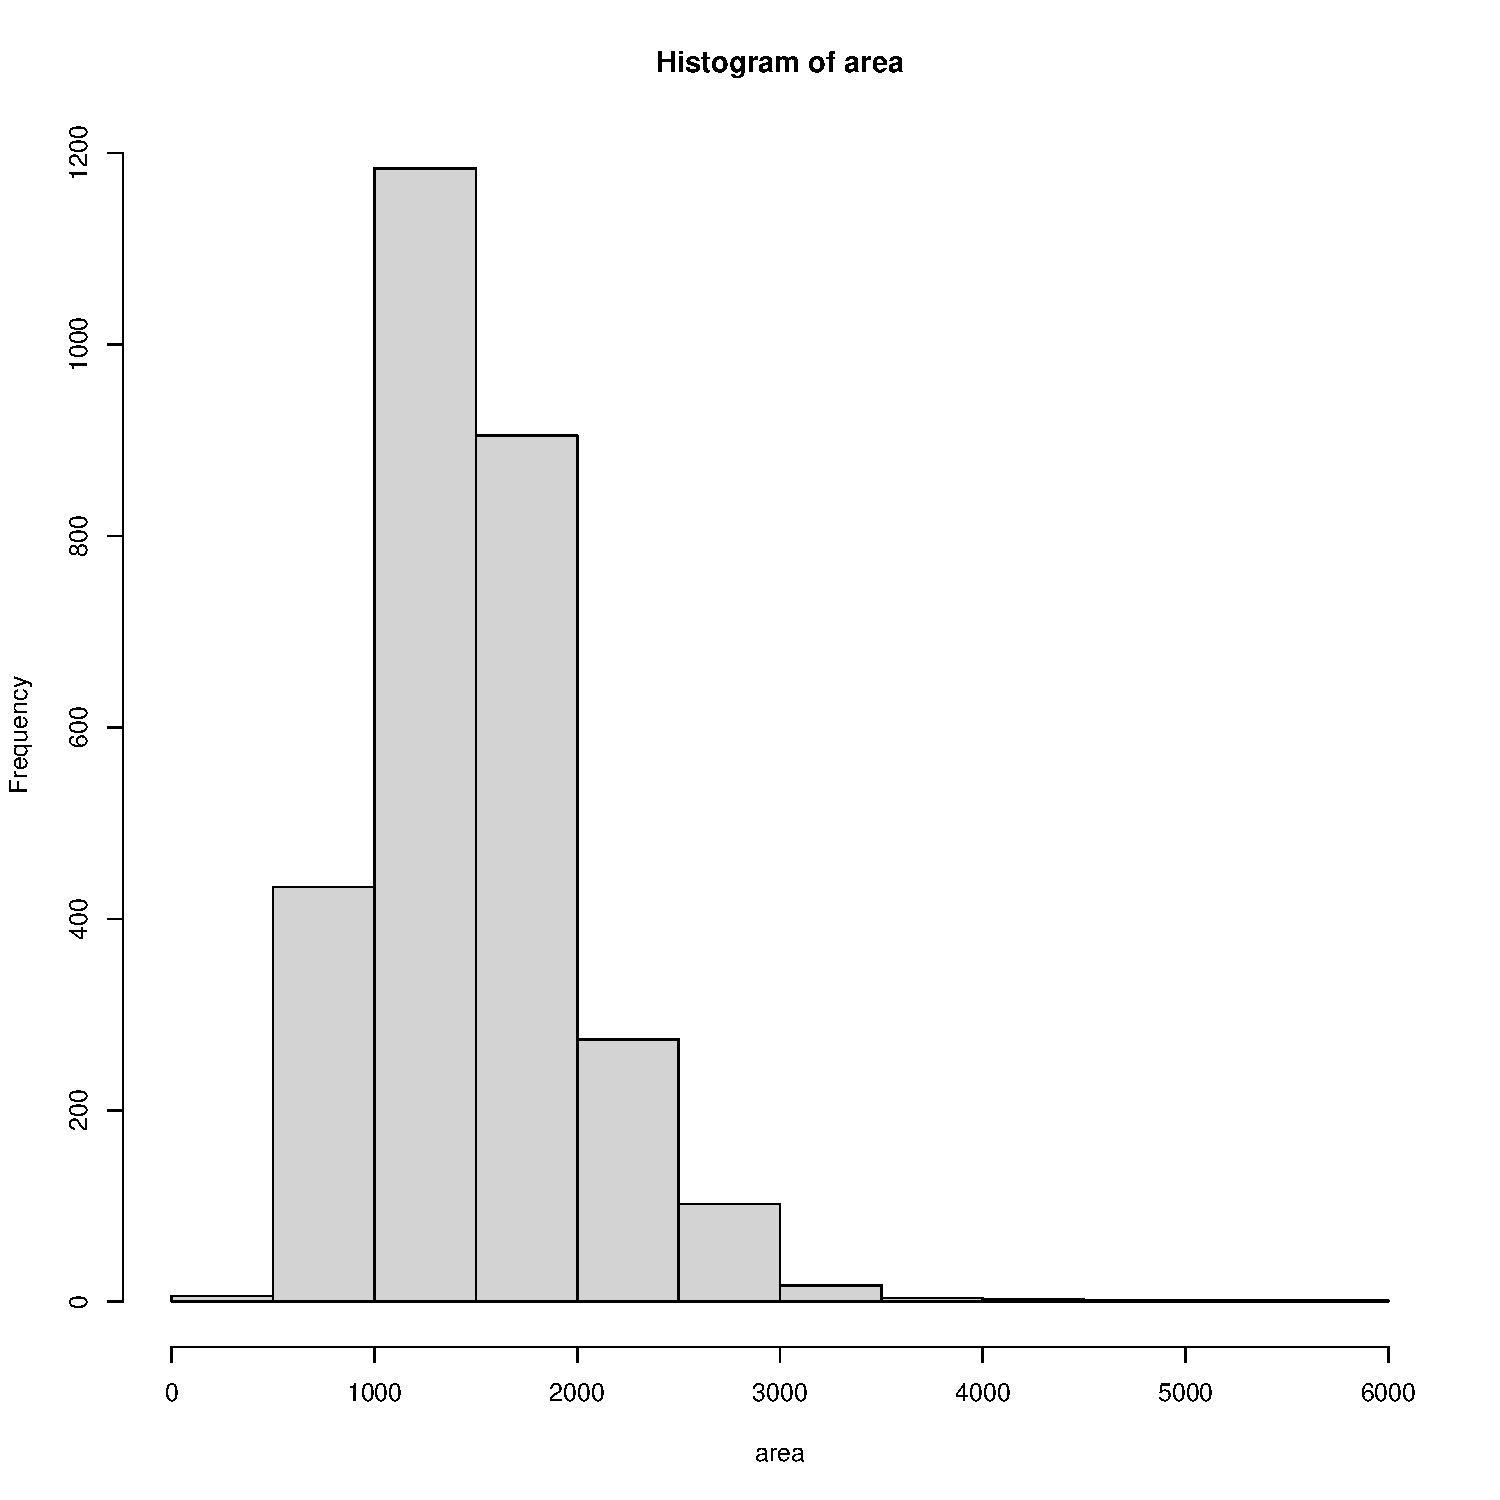
\includegraphics[width=0.65\textwidth]{../area_hist.pdf}
\end{figure}
Her kan vi se at fordelingen er højreskæv, samt at den har den karakteristiske
klokkeform som kendetegner normalfordelingen. 

\section{Den ukendte prøveudtagningsfordeling}
Vi tager stikprøve med \texttt{samp1 <- sample(area,50)}. Her får vi 50
tilfældige værdier. 
\begin{figure}[H]
  \centering
  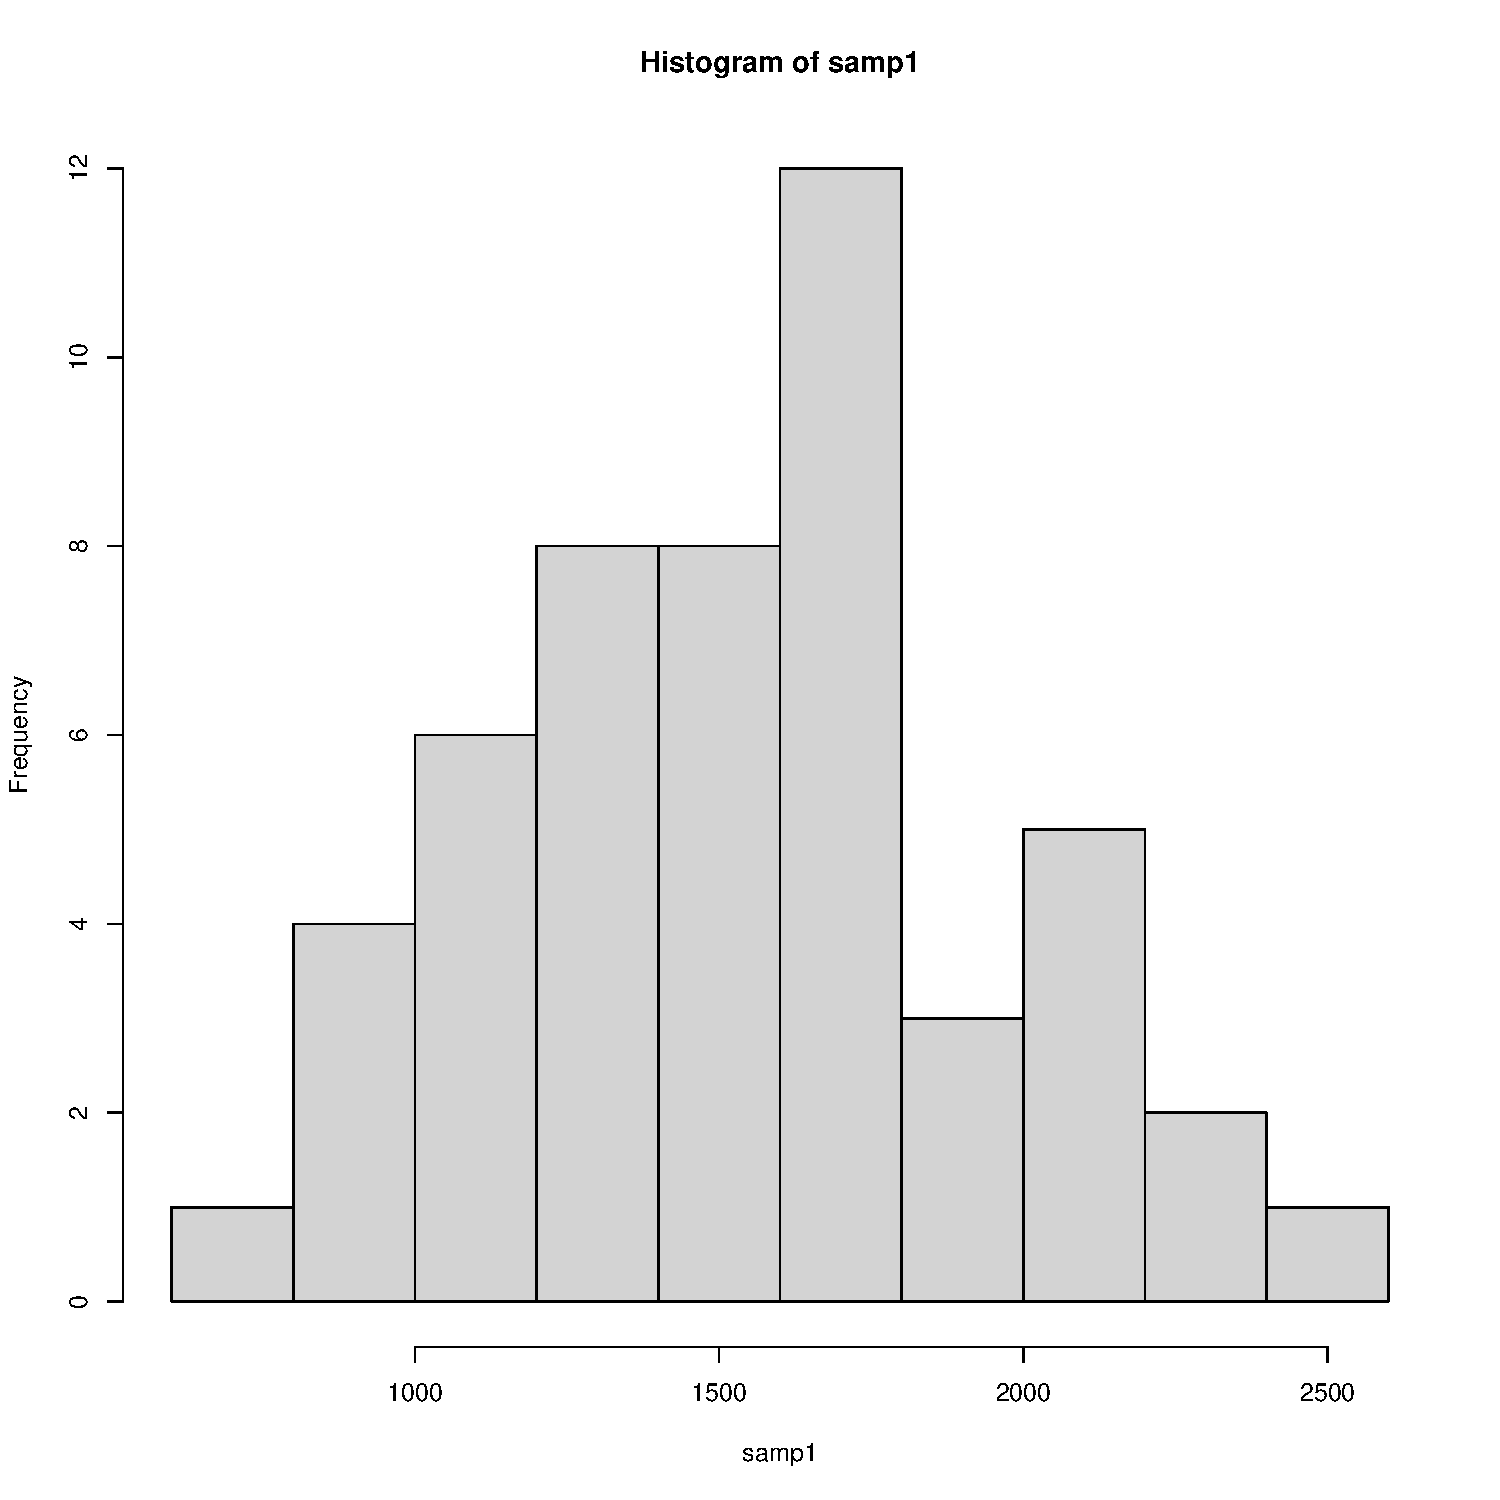
\includegraphics[width=0.65\textwidth]{../sample_area_hist.pdf}
\end{figure}
Fordelingen ligner tilnærmelsesvist en normalfordeling. Fordelingen kan ikke
betegnes som værende højreskæv eller venstreskæv, men derimod symmetrisk.

Vi tager et gennemsnit af \texttt{samp1}, som en approksimering af gennemsnittet
for den generelle population. Dette gennemsnit er 1520 sq ft, hvor  gennemsnittet for
den generelle population er 1499 sq ft. 

Vi tager endnu en stikprøve fra populationen.
\begin{lstlisting}[basicstyle=\ttfamily,language=R]
@> samp2 <- sample(area,50)
@> mean(samp2)
[1] 1489.94
\end{lstlisting}
Denne stikprøve ligger heller ikke langt fra gennemsnit for den generelle
population, den ligger heller ikke langt fra \texttt{samp1}. Den største prøve
vil give et mest nøjagtige skøn, dette er dog ikke at foretrække, da fordelene i
at få 1000 stikprøver frem for 50 stikprøver, ikke giver en meget bedre model.

\subsection{5000 stikprøver}
Vi genererer 5000 stikprøver og tager gennemsnittet.
\lstinputlisting[firstline=28, lastline=33, basicstyle=\ttfamily]{../ex5.R}
Der er 5000 elementer i \texttt{sample\_means50}.
\begin{figure}[H]
  \centering
  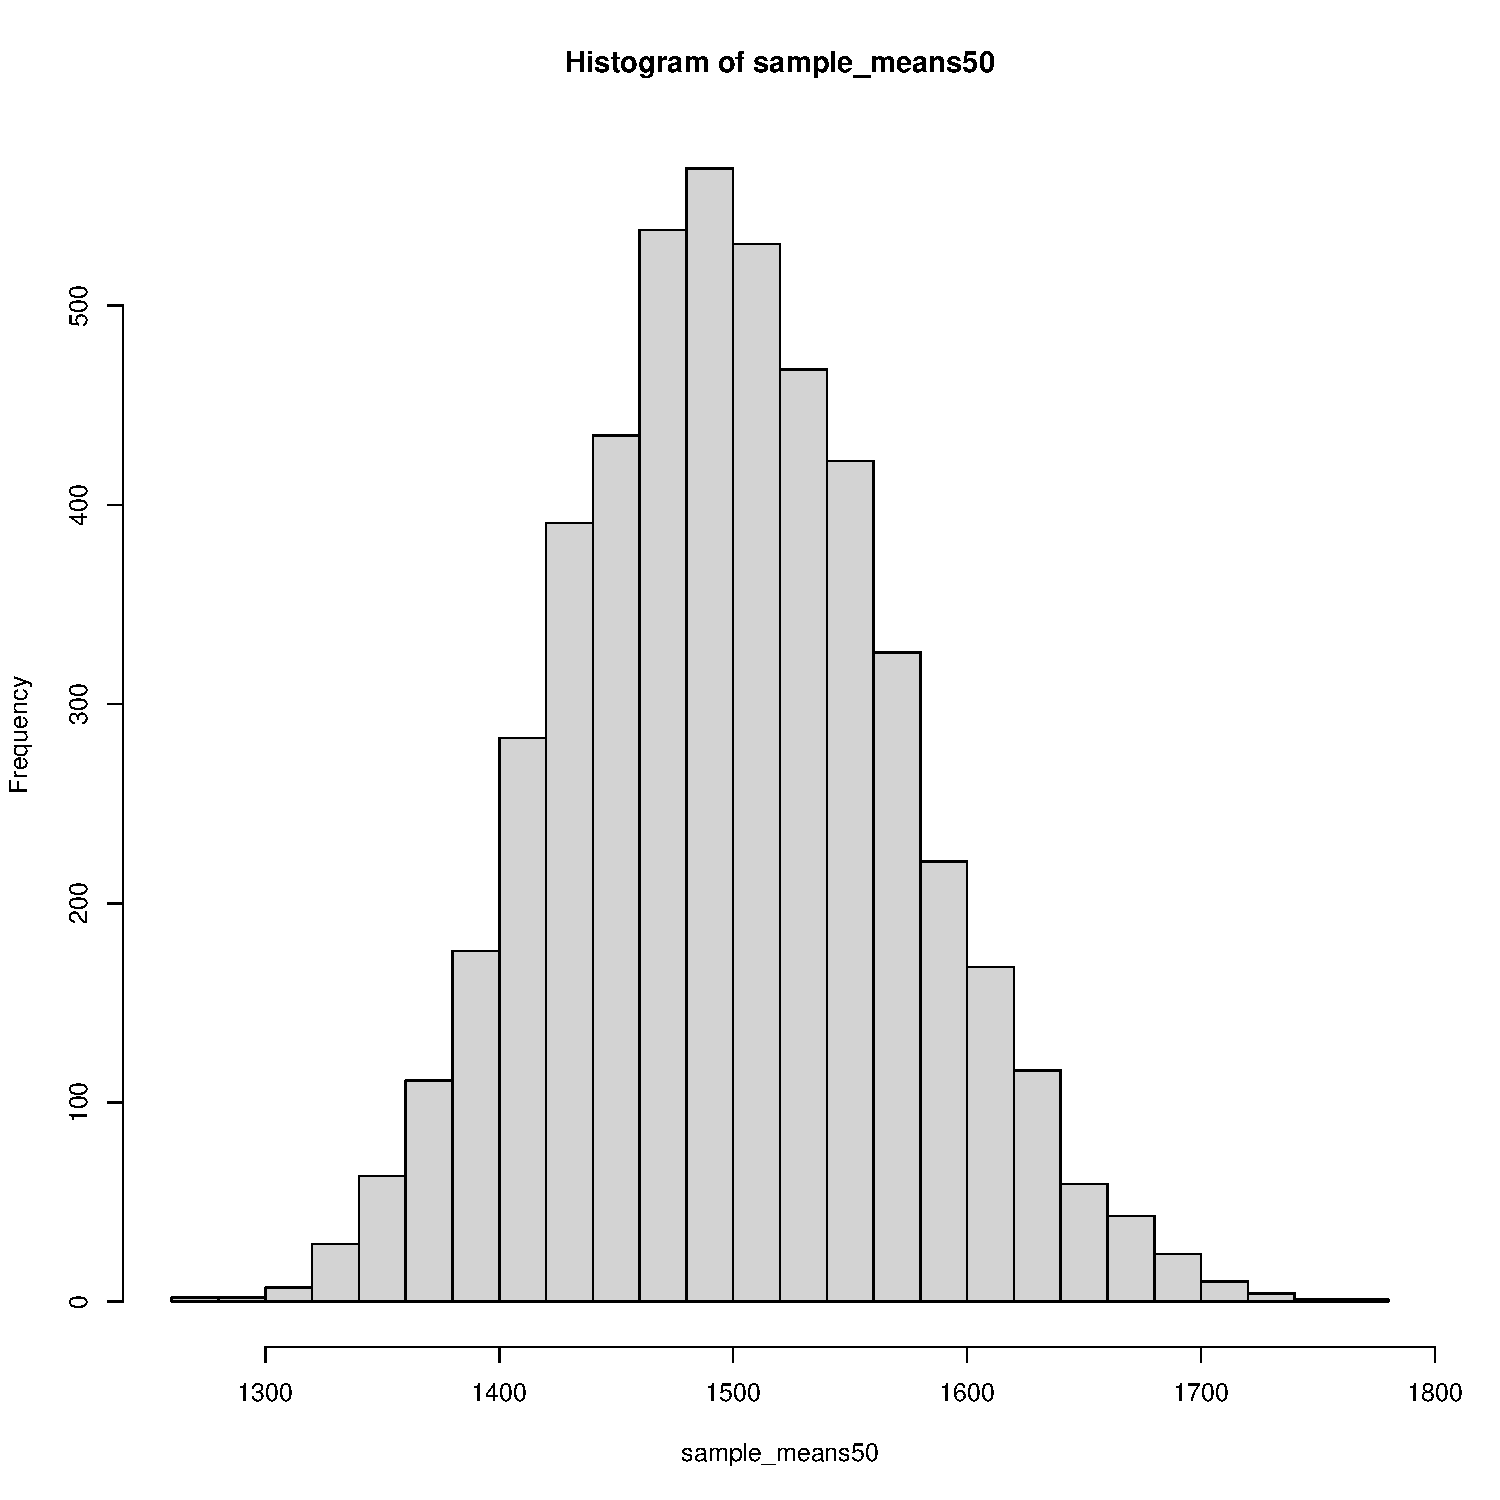
\includegraphics[width=0.65\textwidth]{../sample_means50.pdf}
\end{figure}
Gennesnittet for de 5000 prøver er 
\begin{lstlisting}
@> mean(sample_means50)
[1] 1498.804
\end{lstlisting}

\begin{figure}[H]
  \centering
  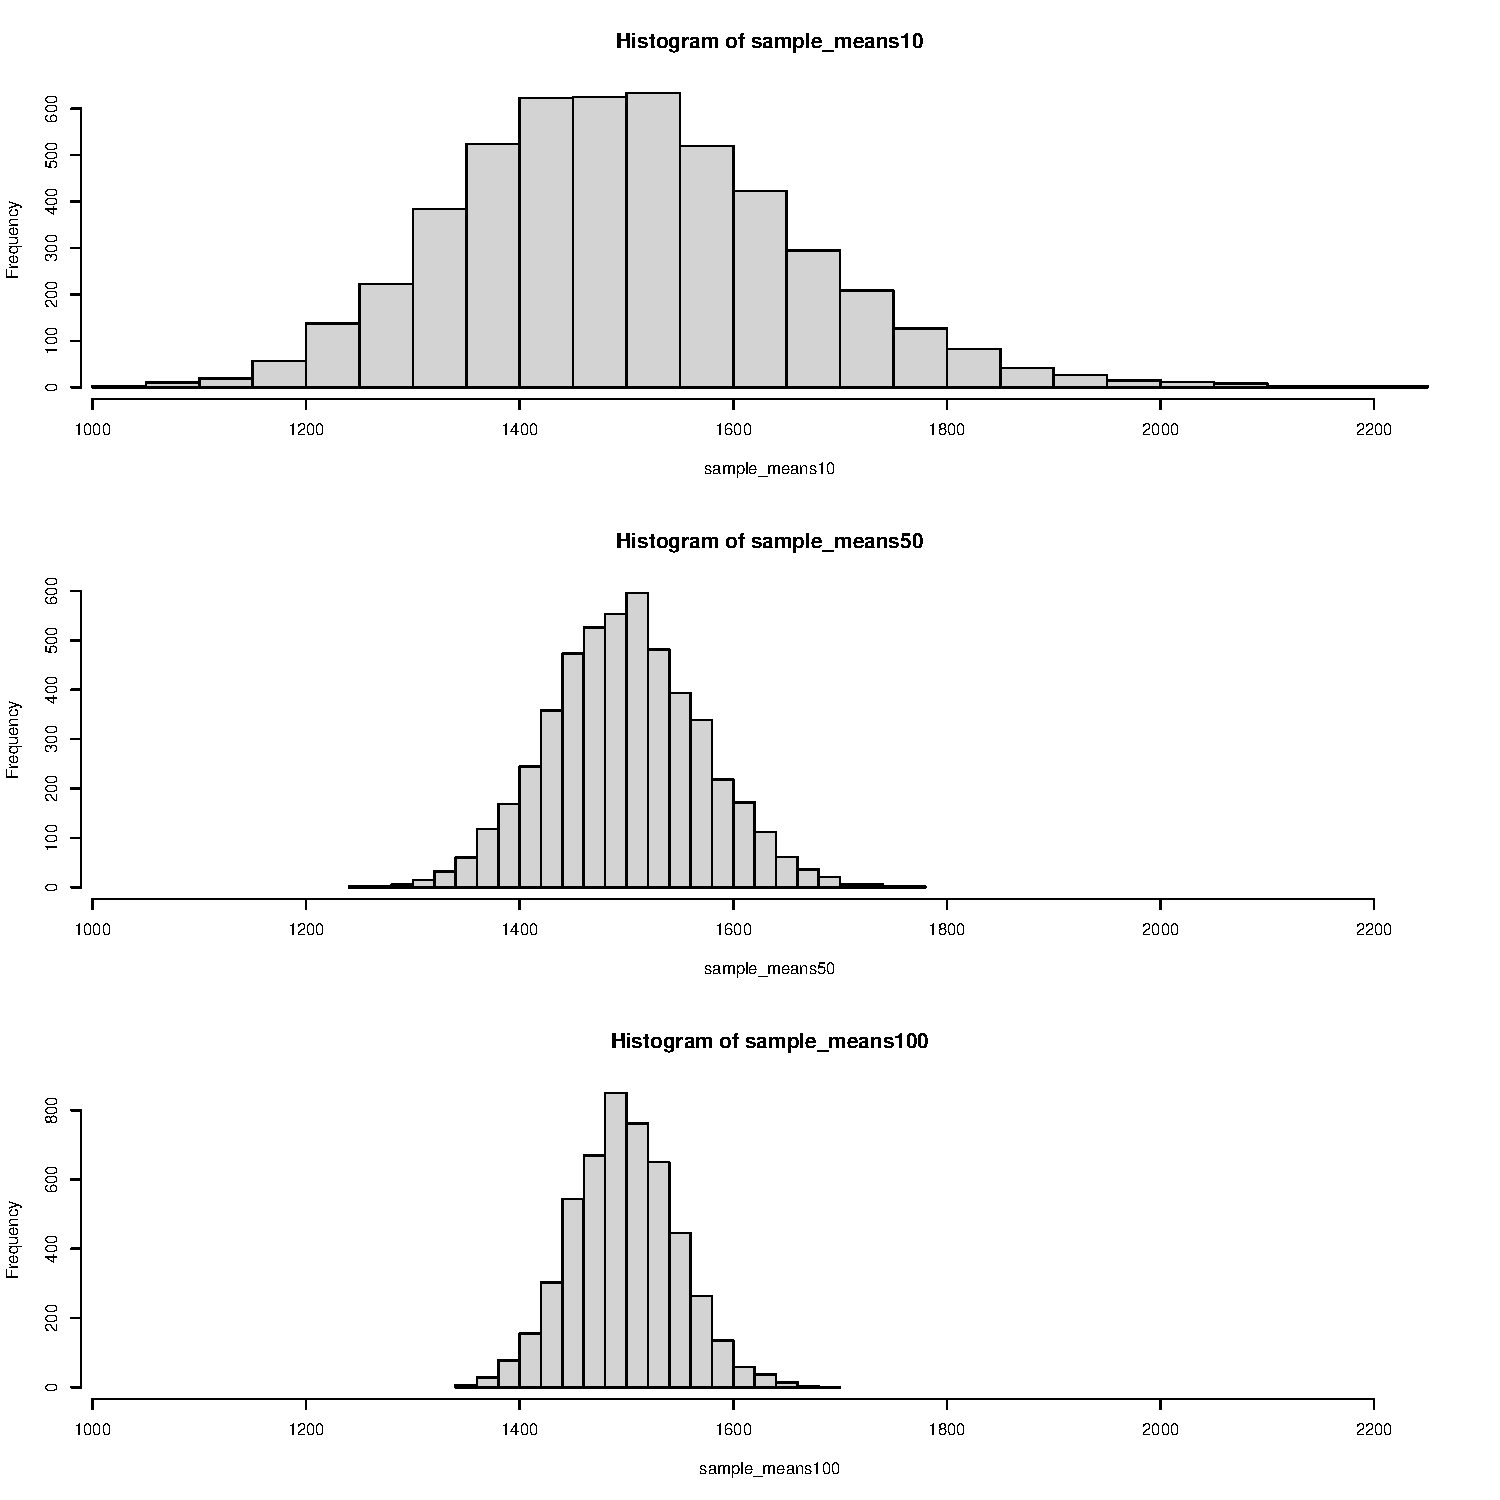
\includegraphics[width=0.65\textwidth]{../sample_means_all.pdf}
\end{figure}
Jo større stikprøvestørrelsen bliver, jo tættere bliver spredningen omkring
middelværdien for den generelle population. Spredningen af data bliver mindre,
siden vi har flere datapunkter med per værdi. Det vil sige at en værdi i
means\_100 generelt set bedre repræsentere end en vilkårlig værdi i means\_10.


\section{Opgaver}

\subsection{1}
Vi tager en stikprøve med \texttt{@> sampPrice <- sample(price, 50)}, et
punktestimat er: 
\begin{lstlisting}
@> mean(sampPrice)
[1] 176008.1
\end{lstlisting}

\subsection{2}
\begin{figure}[H]
  \centering
  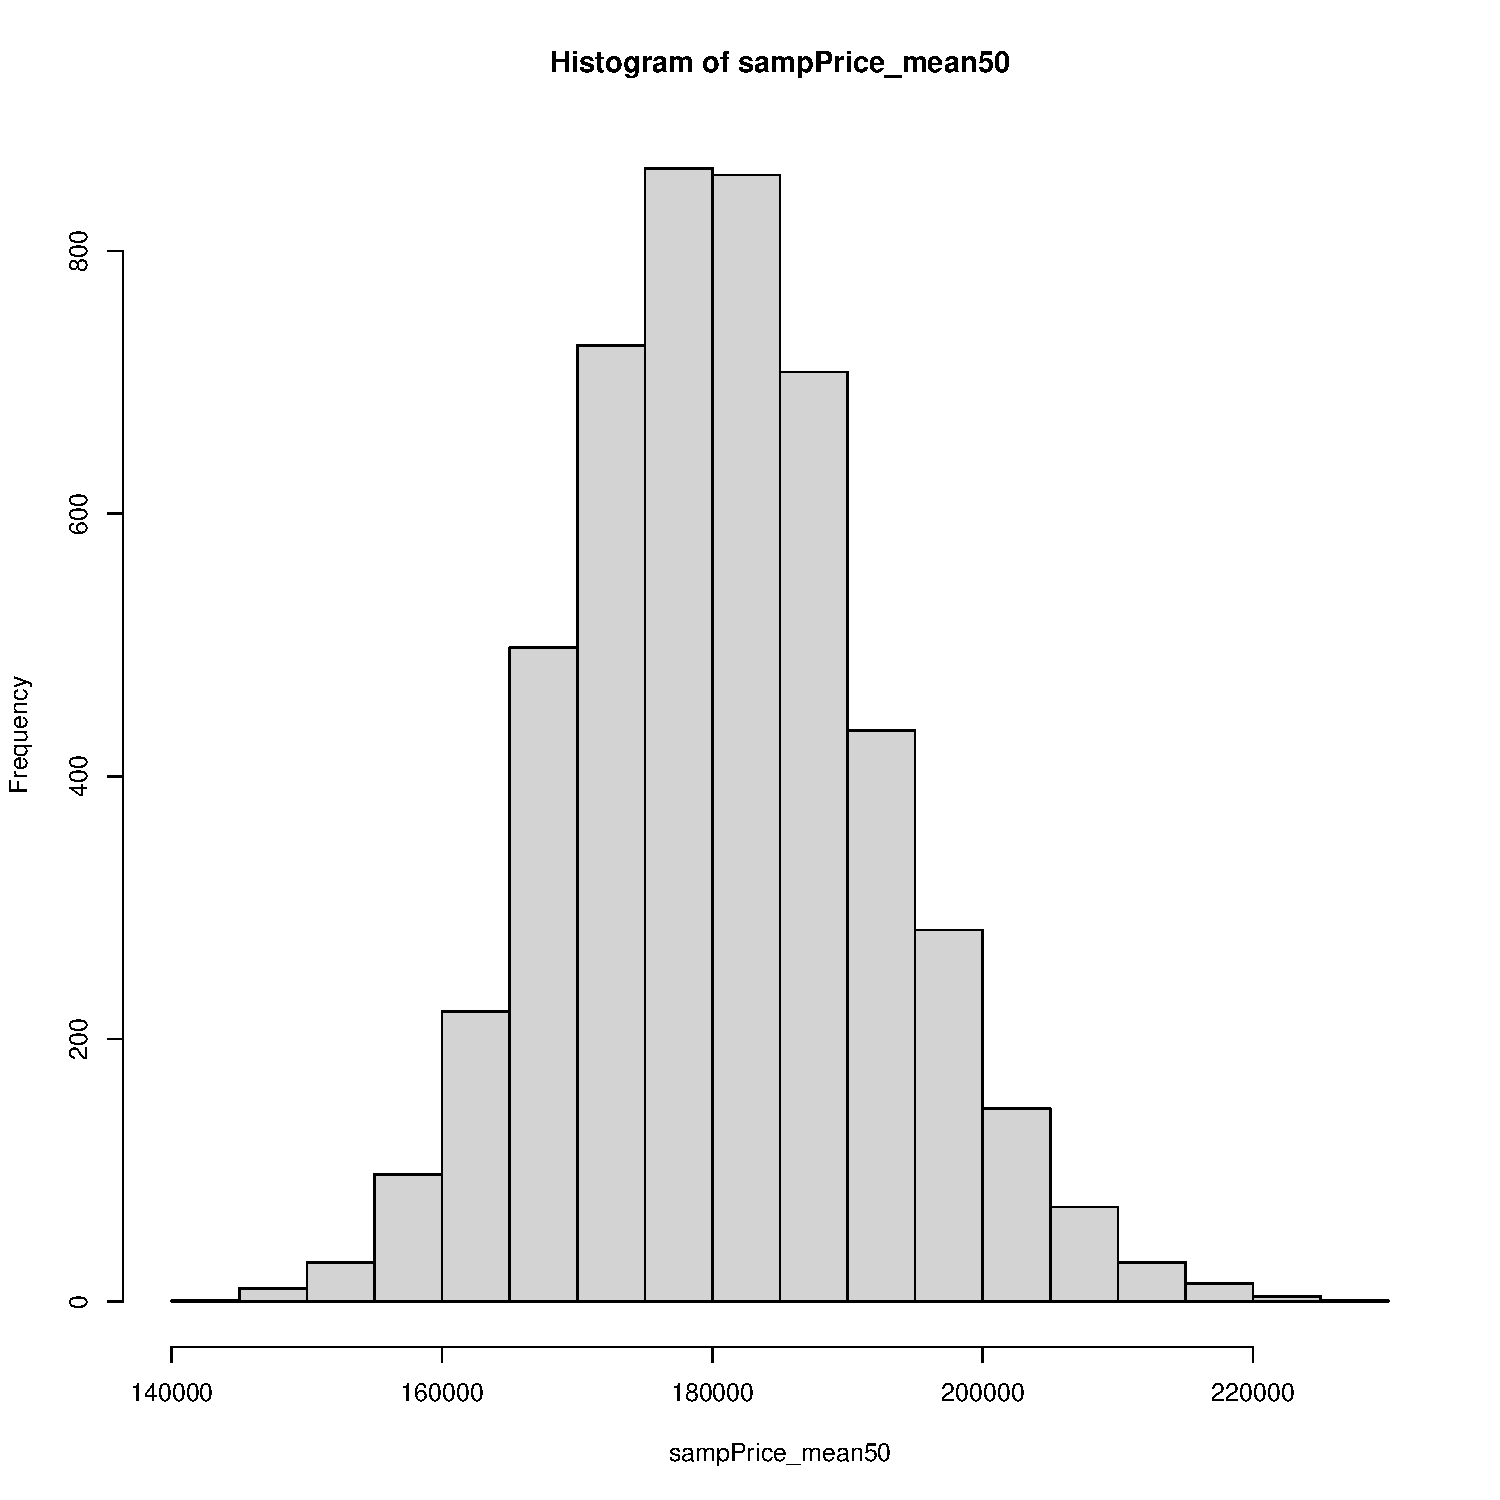
\includegraphics[width=0.65\textwidth]{../sampPrice_mean50.pdf}
  \caption{\texttt{Sample price mean}}
\end{figure}

\begin{lstlisting}[basicstyle=\ttfamily, language=R,
keywordstyle=\color{blue}\bfseries, rulecolor=\color{black}, stringstyle=\color{green}]
sampPrice_mean50 <- rep(NA, 5000)

for(i in 1:5000) {
  samp <- sample(price, 50)
  sampPrice_mean50[i] <- mean(samp)
}
\end{lstlisting}
Fordeling er normalfordelt, med en klokkeform. Ud fra histogrammet, kan det ses
at middelværdien ligger omkring 18000\$. Den reelle middelværdi for hele
populationen er 
\begin{lstlisting}[basicstyle=\ttfamily, language=R, keywordstyle=\color{blue}\bfseries, rulecolor=\color{black}]
@> mean(price)
[1] 180796.1
\end{lstlisting}

\section{3}
Vi laver en fordeling med stikprøvestørrelse på 150, for at kunne sammenligne:
\begin{figure}[H]
  \centering
  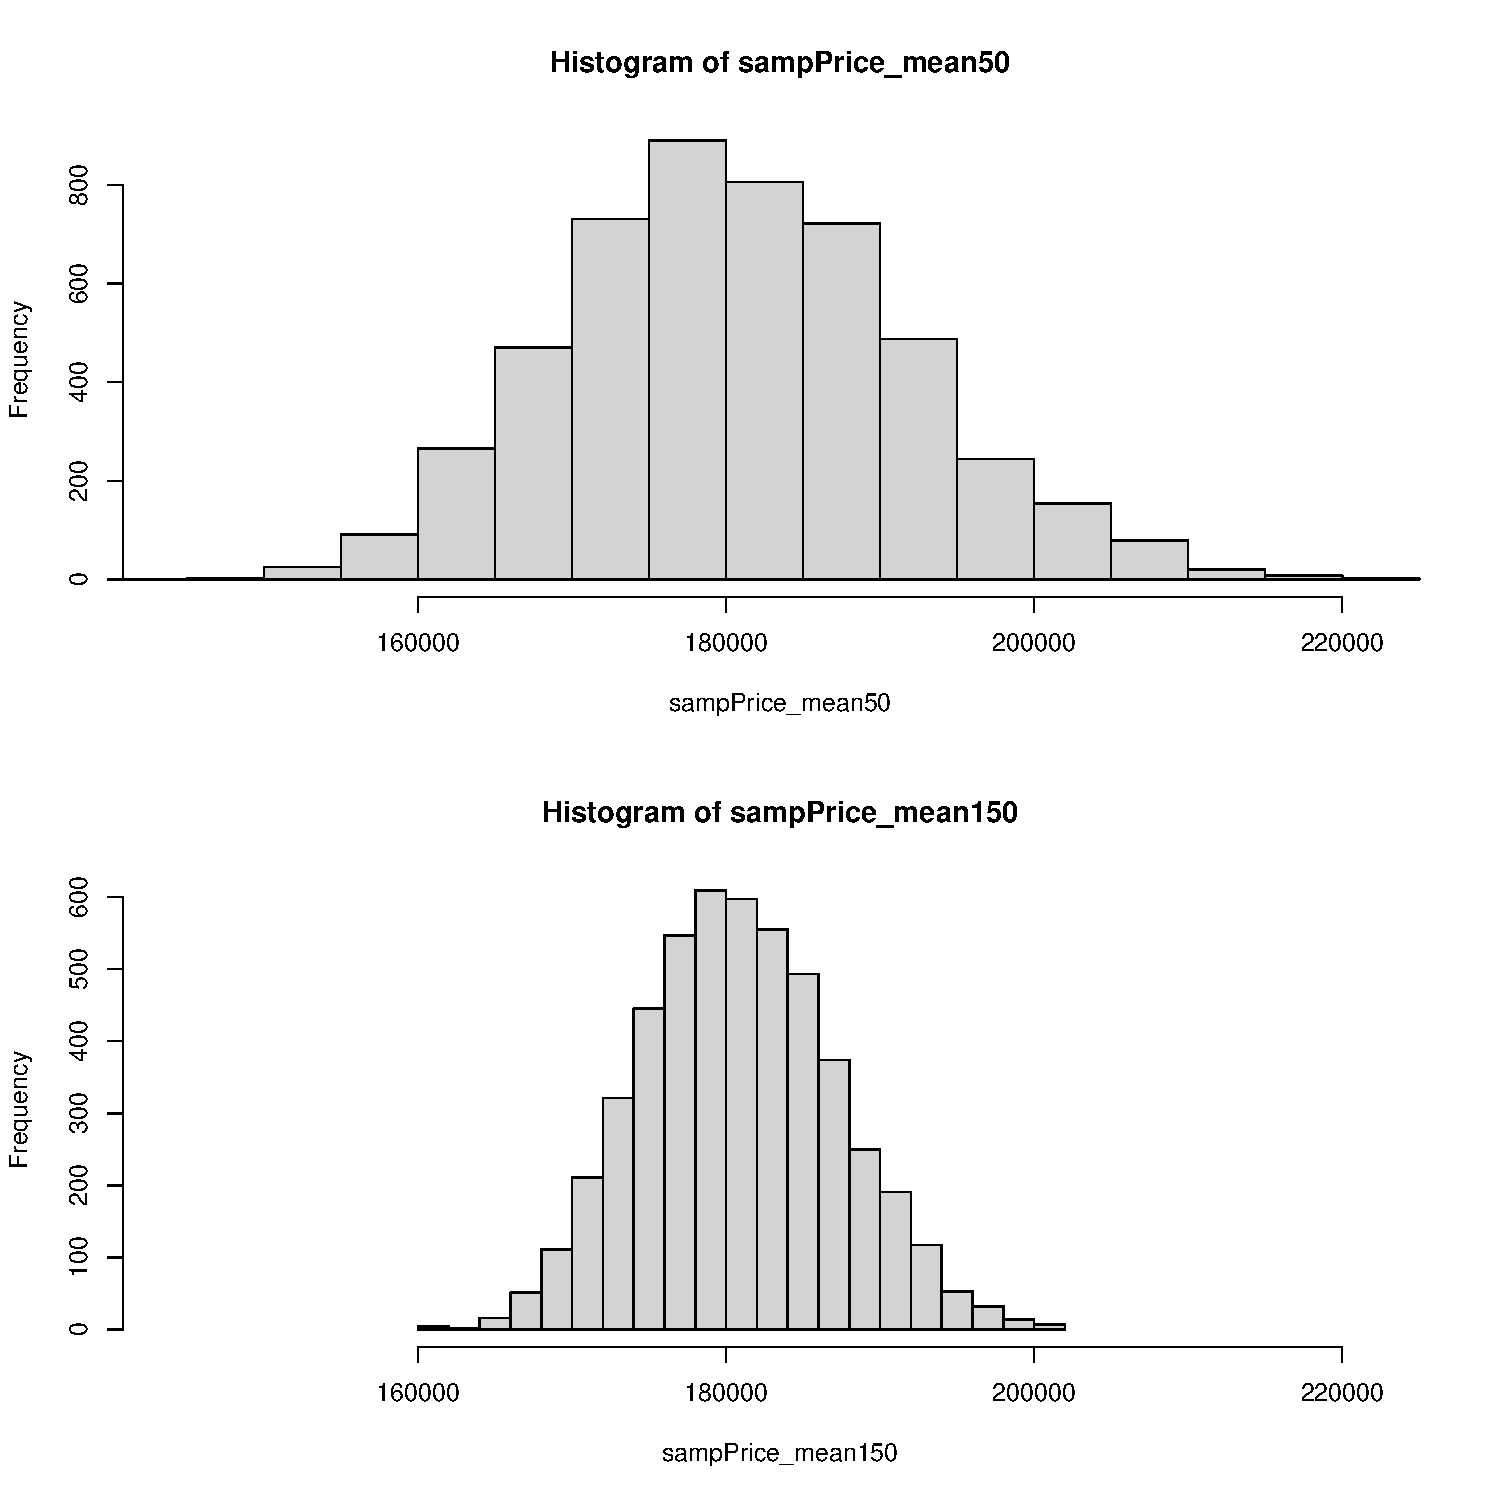
\includegraphics[width=0.65\textwidth]{../pricesample_means_all.pdf}
  \caption{Priser for et område med forskellige stikprøvestørrelser}
\end{figure}
Fordelingen med en stikprøvestørrelse på 150, har en pænere klokkeform end den
med \\stikprøvestørrelse på 50. Spredningen for den med 150 prøver er mindre, og
giver derfor prøve for prøve et bedre billede af data, end den med en
stikprøvestørrelse på 50. Vi vil derfor gerne have en stikprøve af en hvis
størrelse. 


\end{document}

